\chapter{波、量子化模式與產生算符}

\section{波、場與複指數}

量子場論是粒子物理學的基本工具。在初步介紹量子場之前，先整理連結波與粒子的數學事實很有幫助。波本身就是一種場的組態：場在空間中逐點變化，而波則是場值振盪並傳播的一種組態。量子力學提供了這類波與粒子之間的連結。

這裡假定讀者已具備量子力學與狹義相對論的背景知識。本節的直接目的，是回顧粒子物理學所需的部分內容，而非取代這兩門學科的課程。

指數函數的特徵是按比例增長。若
\begin{equation}
f(x)=e^{\alpha x},
\end{equation}
則
\begin{equation}
\frac{df}{dx}=\alpha f.
\end{equation}
在很小的區間內，增量與原有的量成正比。培養皿中的族群增長是個熟悉的例子：個體越多，可繁殖的個體就越多，因此增長率與族群本身成正比。將 \(e^{\alpha x}\) 乘上一個整體常數，並不會改變這項定義性質。

正弦與餘弦會振盪，而不會增長。它們是同一條曲線相差四分之一週期的平移，微分後則會彼此轉換：
\begin{align}
\frac{d}{dx}\sin(kx)&=k\cos(kx),\\
\frac{d}{dx}\cos(kx)&=-k\sin(kx).
\end{align}
單獨來看，兩個函數都不是指數函數，因為其中一個函數的導數與另一個函數成正比。不過，複數線性組合確實具有指數函數的性質。令 \(i^2=-1\)，
\begin{align}
\frac{d}{dx}\bigl(\cos(kx)+i\sin(kx)\bigr)
&=-k\sin(kx)+ik\cos(kx)\\
&=ik\bigl(\cos(kx)+i\sin(kx)\bigr).
\end{align}
因此
\begin{equation}
e^{ikx}=\cos(kx)+i\sin(kx).
\end{equation}
這個恆等式一再出現，因為正弦和餘弦描述了波動式的振盪。當 \(x\) 是空間座標時，函數會隨空間振盪；當自變數是時間時，函數則會隨時間振盪。

\section{頻率、波長與光子動量}

普通頻率 \(f\) 是每秒完成的週期數。一個週期就是一次完整的振盪。角頻率以每秒幾弧度來量度相同的運動：
\begin{equation}
\omega=2\pi f.
\end{equation}
這兩種記法描述的是同一個頻率。計算時有時會在兩者之間轉換，以免出現不必要的 \(2\pi\) 因子；不過，這些因子終究不會完全消失。

波長 \(\lambda\) 是一個完整空間週期所占的距離。若波以速率 \(v\) 傳播，則每個週期的距離乘上每秒的週期數，便是傳播速率：
\begin{equation}
\lambda f=v.
\end{equation}
對真空中的光而言，\(v=c\)，因此
\begin{equation}
\lambda f=c.
\end{equation}
聲波的等式右側是聲速；水波則是相應的水波速率。因此，出現 \(c\) 是光的性質，並非所有波都適用的定義。

量子力學以兩種記法引入普朗克常數：
\begin{equation}
\hbar=\frac{h}{2\pi}.
\end{equation}
從 \(h\) 改用 \(\hbar\)，只不過是把 \(2\pi\) 因子從一個方程式移到另一個方程式。

有量綱常數的數值取決於表示它們時所用的單位。公尺、秒和公斤是符合人類尺度的慣用單位，方便描述日常的長度與時間。以手臂長度為基準的傳統單位，曾適用於布料或繩索；無論公尺的歷史沿革究竟如何，都沒有基本原理會特別選定這種符合人類尺度的單位。在 SI 單位制中，
\begin{equation}
\begin{aligned}
h &\simeq 6.6\times10^{-34}\ \mathrm{J\,s},
&\hbar &\simeq 1.1\times10^{-34}\ \mathrm{J\,s},\\
c &\simeq 3\times10^8\ \mathrm{m\,s^{-1}}.
\end{aligned}
\end{equation}
這些數值要表達的是它們在慣用單位下的尺度：普朗克常數極小，而光速極大。

一個模式中的單一量子具有能量
\begin{equation}
E_{\text{one quantum}}=\hbar\omega=hf.
\end{equation}
這是單一光子的能量，並非任意經典電磁波的總能量。可見光的頻率約為每秒 \(10^{15}\) 個週期，因此典型光學光子的能量約為
\begin{equation}
E_\gamma\sim 10^{-19}\ \mathrm{J}.
\end{equation}
光學振盪即使如此迅速，每個量子的能量仍極小，因為 \(h\) 非常小。因此，宏觀尺度的光能包含數量極其龐大的光子。

能量和動量特別值得注意，因為兩者都是守恆量。它們是有用的帳目：進入某個過程的總能量與總動量，必須和離開該過程的總能量與總動量相平衡。動量是向量，方向與運動方向相同。對於運動速度遠低於光速的粒子，
\begin{equation}
\vec p=m\vec v.
\end{equation}

現在考慮沿單一方向準直傳播、而非向許多方向散開的電磁輻射。它的動量沿著光束方向。非相對論公式不能用於光子，因為 \(m\) 表示靜止質量，而光子的靜止質量為零。儘管如此，有個實用的量綱助記法：若 \emph{不恰當地}把 \(E/c^2\) 當成質量賦予光子，再代入 \(v=c\)，就會得到
\begin{equation}
mv\longrightarrow \frac{E}{c^2}c=\frac{E}{c}.
\end{equation}
這個做法碰巧得到正確答案，量綱也正確，但不能據此合理地論證光子具有靜止質量 \(E/c^2\)。準直輻射的正確相對論敘述是
\begin{equation}
|\vec p|=\frac{E}{c}.
\end{equation}
這個方程式給出動量的大小；動量方向則與輻射傳播方向相同。

對單一光子而言，
\begin{align}
|\vec p_\gamma|
&=\frac{E_\gamma}{c}
=\frac{hf}{c}.
\end{align}
對光而言，
\begin{equation}
\lambda f=c,
\qquad
\frac{f}{c}=\frac{1}{\lambda},
\end{equation}
因此
\begin{equation}
|\vec p_\gamma|=\frac{hf}{c}=\frac{h}{\lambda}.
\end{equation}

\begin{figure}[t]
\centering
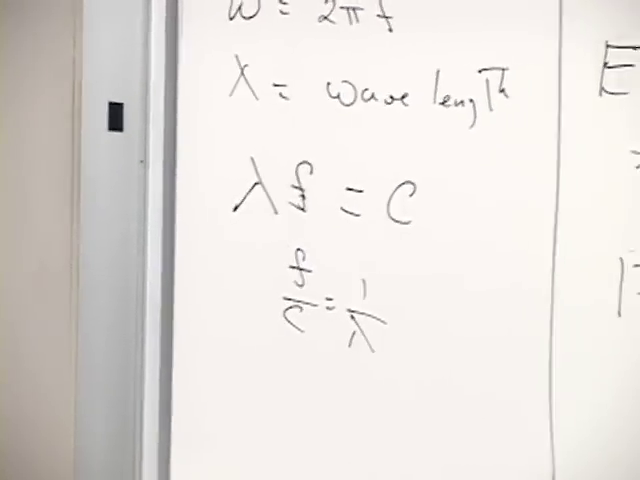
\includegraphics[width=0.56\textwidth]{lecture_02_figure_02.png}
\caption{對光而言，\(\lambda f=c\)與\(f/c=1/\lambda\)，便可得到\(|\vec p_\gamma|=h/\lambda\)。}
\lectureframe{00:21:39}
\end{figure}

波長越短，光子動量越大。這是粒子物理學中最重要的量子事實之一。要研究微小物體，需要以短波長作為探測；短波長所付出的代價，就是較大的動量。

\begin{classroomqa}
\lecturetimestamp{00:22:23}
\audiencequestion{\(E=\hbar\omega\)是基本原理，還是可以從更深層的原理推導出來？}
\lecturerresponse{這個結果可由諧振子的量子力學推導而得。這裡會直接使用此結果，不再重複證明；下文建立的振子描述，會說明它更深層的背景。}
\end{classroomqa}


\section{波的振幅與光子數}

\begin{classroomqa}
\lecturetimestamp{00:23:10}
\audiencequestion{以光子的語言來說，波的振幅代表什麼？}
\lecturerresponse{比較兩個波長和頻率相同、但振幅不同的波，例如 \(\sin(kx)\) 和 \(A\sin(kx)\)。在經典物理中，固定區域內的能量與振幅平方成正比。在量子力學中，含有 \(n\) 個光子的模式具有能量 \(n\hbar\omega\)。因此，在頻率、區域和正規化方式都固定時，振幅的量級會隨 \(\sqrt n\) 增長。}
\end{classroomqa}

兩個波的振盪型態完全相同，只是一個比另一個強。\footnote{示意圖參照 00 至 23 的波形比較：47--00至24：28。}

\begin{figure}[t]
\centering
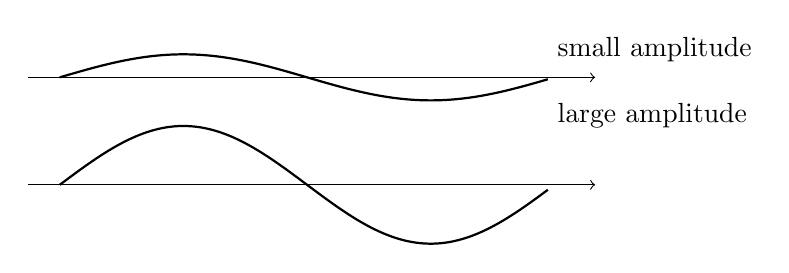
\begin{tikzpicture}[x=1cm,y=0.65cm]
\draw[->] (-0.4,0) -- (6.8,0);
\draw[->] (-0.4,-2.1) -- (6.8,-2.1);
\draw[thick] plot[domain=0:6.2,samples=120] (\x,{0.45*sin(\x r)});
\draw[thick] plot[domain=0:6.2,samples=120] (\x,{-2.1+1.15*sin(\x r)});
\draw (6.2,0.55) node[right]{small amplitude};
\draw (6.2,-0.75) node[right]{large amplitude};
\end{tikzpicture}
\caption{波長與頻率相同、振幅不同的波。}
\end{figure}

對固定的波量而言，
\begin{equation}
E_{\text{wave}}\propto A^2.
\end{equation}
對電磁波來說，這就是熟知的場能與場強平方成正比。如果同一個模式含有 \(n\) 個光子，那麼
\begin{equation}
E_{\text{wave}}=n\hbar\omega.
\end{equation}
因此，在模式、頻率、正規化方式和區域都固定時，
\begin{equation}
A^2\propto n\hbar\omega,
\qquad
A\propto\sqrt n\quad\text{at fixed }\omega.
\end{equation}
這裡並未主張任何精確的正規化關係。波的涵蓋範圍很重要：將原本均勻的波長度加倍，會改變總能量，卻不會改變局部振幅。因此，這個正比關係應理解為適用於固定區域，例如一個波長。

此外，量子力學還有一項特有的限制：振幅和相位不能同時具有精確的經典值。因此，若問題 ``單一光子的振幅是多少？'' 要求的是完全確定的經典場，便沒有明確答案。不過，令 \(n=1\) 仍可得到合理的量級估計。

\begin{classroomqa}
\lecturetimestamp{00:28:25}
\audiencequestion{電磁波圖中的垂直位移代表光子在空間中的位置嗎？}
\lecturerresponse{不代表。傳播軸是空間座標，而垂直座標表示電場或磁場的值。動量沿傳播軸方向，不是沿圖中場振幅的方向。}
\end{classroomqa}

波可以沿任意空間方向傳播，但熟悉的正弦波圖只把水平軸當作空間座標。圖中另一個方向表示場強。

\begin{classroomqa}
\lecturetimestamp{00:29:37}
\audiencequestion{所說的光子數，是在一個波長或一個週期內計算的嗎？}
\lecturerresponse{可以選定一個固定區域，例如一個波長。這就是為什麼此處只有正比關係：總能量和光子數也取決於涵蓋了多少波。在振幅相同的情況下，涵蓋兩個、三個或四個波長，能量就相應增加。}
\end{classroomqa}

\begin{classroomqa}
\lecturetimestamp{00:30:17}
\audiencequestion{單一光子的振幅沒有意義嗎？}
\lecturerresponse{只有在令 \(n=1\) 後，將其視為量級估計，才有意義。對電磁模式而言，電場和磁場資訊的作用類似於共軛的位置與動量資訊，因此量子不確定性限制了經典振幅能指定得多精確。量級關係仍然有用。}
\end{classroomqa}

這些問題已經引向量子場論；在量子場論中，場變數與粒子數之間的關係可以精確表述。目前只需掌握這些正比關係。

\section{一般量子關係與慢速物質波}

有些為光子引入的公式適用範圍更廣，有些則不然。在討論電子之前，值得先釐清各公式的適用範圍。

\begin{figure}[t]
\centering
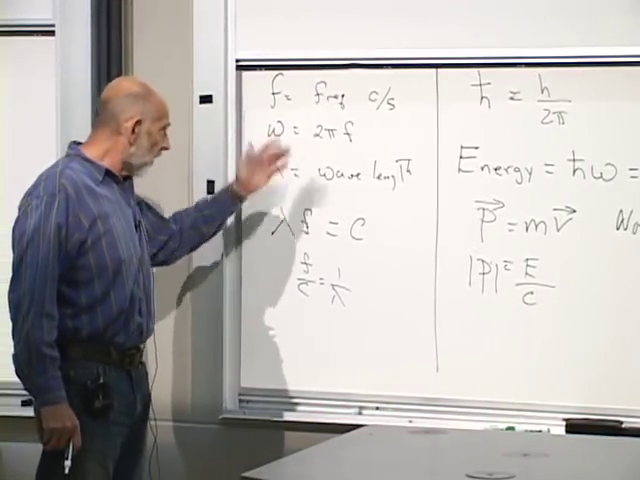
\includegraphics[width=0.82\textwidth]{lecture_02_figure_03.png}
\caption{波的定義，以及光子與非相對論動量關係的適用範圍比較。}
\lectureframe{00:31:52}
\end{figure}

\(f\)、\(\omega=2\pi f\)和\(\lambda\)的定義普遍適用。在此處的討論中，量子關係
\begin{equation}
E=\hbar\omega=hf
\end{equation}
也普遍適用。相較之下，含有 \(c\) 的公式，例如 \(\lambda f=c\) 和 \(|\vec p|=E/c\)，適用於以光速傳播的波。公式 \(\vec p=m\vec v\) 則適用於運動速度遠低於光速的粒子。介於這兩種情形之間的相對論運動，需要用到目前還不必介紹的插值公式。

動量--波長關係在光子的例子中仍然成立：
\begin{equation}
p=\frac{h}{\lambda}.
\end{equation}
這裡的 \(p\) 表示大小，並假設 \(\lambda\) 是正的波長；方向可以另外指定。

\begin{figure}[t]
\centering
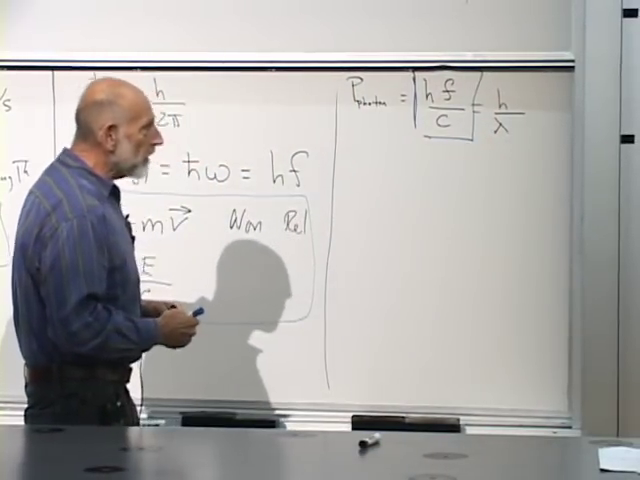
\includegraphics[width=0.74\textwidth]{lecture_02_figure_04.png}
\caption{光子動量 \(|\vec p_\gamma|=hf/c=h/\lambda\)，由此得到一般的德布羅意關係。}
\lectureframe{00:33:32}
\end{figure}

電子、原子核，甚至保齡球都可以與波相聯繫。電子干涉就是這個事實的一種表現。將電子波寫成 \(\psi\)。對於緩慢運動的電子，什麼關係取代了 \(\lambda f=c\)？缺少的關鍵是能量與動量之間的非相對論關係。

從動能和動量開始：
\begin{align}
E&=\frac12 mv^2,\\
p&=mv,
\qquad
v=\frac{p}{m}.
\end{align}
將最後一個關係代入第一個，得到
\begin{align}
E
&=\frac12m\left(\frac{p}{m}\right)^2\\
&=\frac{p^2}{2m}.
\end{align}
質量在 \(\frac12 mv^2\) 中位於分子，在 \(p^2/(2m)\) 中則位於分母。這兩處很容易混淆，也值得重新推導一次。

現在使用一般的量子關係
\begin{equation}
E=hf,
\qquad
p=\frac{h}{\lambda}.
\end{equation}
對單一慢速粒子而言，
\begin{align}
hf
&=\frac{p^2}{2m}\\
&=\frac{1}{2m}\left(\frac{h}{\lambda}\right)^2\\
&=\frac{h^2}{2m\lambda^2}.
\end{align}
兩邊除以 \(h\)，得到
\begin{equation}
f=\frac{h}{2m\lambda^2}.
\end{equation}

\begin{figure}[t]
\centering
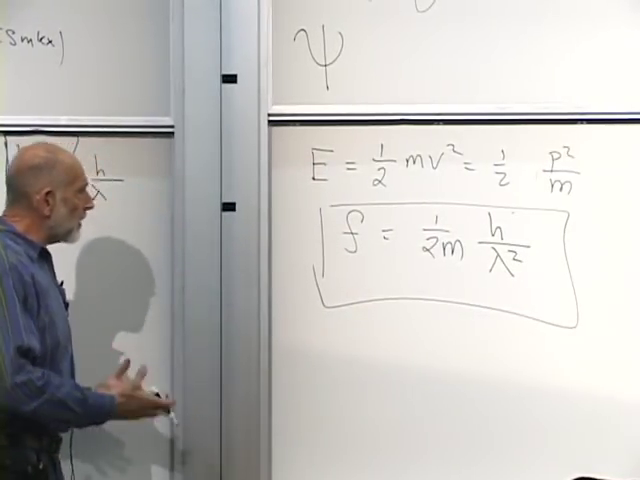
\includegraphics[width=0.64\textwidth]{lecture_02_figure_05.png}
\caption{對慢速粒子而言，\(E=p^2/(2m)\)和\(p=h/\lambda\)可得\(f=h/(2m\lambda^2)\)。}
\lectureframe{00:37:47}
\end{figure}

對光而言，
\begin{equation}
f\propto\frac{1}{\lambda},
\end{equation}
對慢速物質而言，
\begin{equation}
f\propto\frac{1}{\lambda^2}.
\end{equation}
不必孤立地記住第二個關係，隨時都可以由 \(E=p^2/(2m)\)、\(E=hf\) 和 \(p=h/\lambda\) 推導出來。它給出原子中緩慢運動的電子所對應的 Schr\"odinger 波頻率。

\begin{classroomqa}
\lecturetimestamp{00:38:35}
\audiencequestion{非相對論的頻率--波長關係也適用於電子以外的粒子嗎？}
\lecturerresponse{是的。它適用於任何運動速度遠低於光速的粒子。慢速極限與光速極限之間的相對論插值，是另一個主題。}
\end{classroomqa}

\begin{classroomqa}
\lecturetimestamp{00:38:55}
\audiencequestion{哪一個關係適用於中微子？}
\lecturerresponse{要看中微子的速度。自然界中遇到的大多數中微子都以非常接近光速的速度運動，因此光速情形的關係是很好的近似。若中微子的速度遠低於光速，則適用非相對論關係。}
\end{classroomqa}

\editorialnote{中微子問題之後，緊接著有一段簡短的聽眾交流，談到振幅、量子和電子波長的差異，但內容損壞嚴重，無法確實還原。仍可辨認的回答表示，會稍後再討論不同波長的振幅與量子之間的一般關係。}

\begin{classroomqa}
\lecturetimestamp{00:39:56}
\audiencequestion{來自 \(20\,\mathrm{keV}\) 加速器的電子是慢速粒子，還是相對論性粒子？}
\lecturerresponse{這裡將它視為慢速粒子。在 \(c=1\) 單位制中，質量、能量和動量可以用相同單位表示。電子的靜能量級約為 \(0.5\,\mathrm{MeV}\)，而 \(20\,\mathrm{keV}\) 小得多。等價地說，非相對論動量判準是 \(p\ll mc\)。}
\end{classroomqa}

此例中的能量比較為
\begin{equation}
K=20\,\mathrm{keV}\ll m_ec^2\simeq0.5\,\mathrm{MeV}.
\end{equation}
\editorialnote{00處的原文段落：39：56--00：41：40先將 \(20\,\mathrm{keV}\) 作為加速器能量提出，接著以動量和靜質量的比較來表述相對論判準。分別寫出動能判準和動量判準，可以避免把引述的能量等同於動量，同時保留原文所述的非相對論結論。}

\section{相速度、群速度與色散}

\begin{classroomqa}
\lecturetimestamp{00:41:46}
\audiencequestion{頻率乘以波長，能用來求得電子波的速度嗎？}
\lecturerresponse{這樣得到的是相速度，不是電子本身的速度。局域化波包有兩種速度：描述內部波峰和波谷運動的相速度，以及描述包絡運動的群速度。群速度對應於粒子的運動速度。}
\end{classroomqa}

波包在局部看起來像正弦或餘弦波，但受到包絡限制。波包移動時，包絡和其中的波峰不一定以相同速度前進。\footnote{示意圖參照 00 至 42 的波包討論：34--00至44：11。}

\begin{figure}[t]
\centering
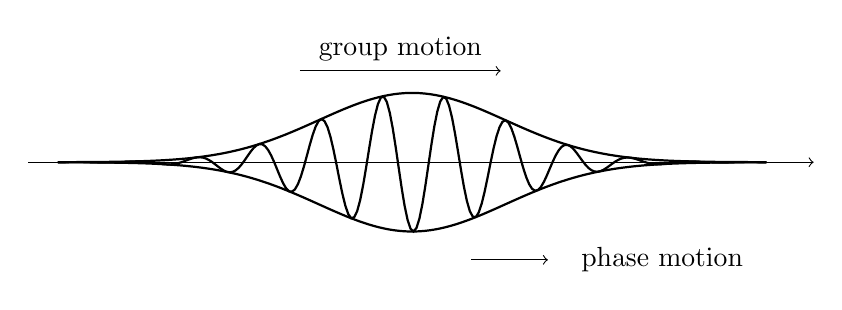
\begin{tikzpicture}[x=0.75cm,y=0.8cm]
\draw[->] (-0.5,0) -- (12.8,0);
\draw[thick] plot[domain=0:12,samples=140] (\x,{1.10*exp(-0.20*(\x-6)^2)});
\draw[thick] plot[domain=0:12,samples=140] (\x,{-1.10*exp(-0.20*(\x-6)^2)});
\draw[thick] plot[domain=0:12,samples=240] (\x,{1.10*exp(-0.20*(\x-6)^2)*sin(6*\x r)});
\draw[->] (4.1,1.45) -- (7.5,1.45);
\draw (5.8,1.8) node{group motion};
\draw[->] (7.0,-1.55) -- (8.3,-1.55);
\draw (8.7,-1.55) node[right]{phase motion};
\end{tikzpicture}
\caption{局域化波包的包絡和內部相位通常以不同速度移動。}
\end{figure}

相速度是單色分量中波峰、波谷和其他固定相位的移動速度。對非相對論性色散關係而言，
\begin{equation}
v_\phi=f\lambda=\frac{h}{2m\lambda}.
\end{equation}
相速度取決於波長。因此，不同波長的分量具有不同的相速度，波峰會在波包內移動，而波包也會發生色散。群速度是整個波包的移動速度，也就是對應於粒子的速度。

有一個簡單的特例：如果所有波長的分量都以相同速度移動，相速度和群速度便相同。真空中的光就具有這項性質：所有波長都以 \(c\) 傳播。慢速粒子的關係則不同；其中的 \(f\lambda\) 會隨 \(\lambda\) 改變。

方程式
\begin{equation}
f=\frac{h}{2m\lambda^2}
\end{equation}
稍加改寫後，就是自由 Schr\"odinger 方程式。頻率決定平面波的時間依賴性，波長決定它的空間依賴性，而 Schr\"odinger 方程式則連結兩者。反過來說，將頻率和波長皆確定的波代入自由 Schr\"odinger 方程式，就會得到這個色散關係。

\begin{classroomqa}
\lecturetimestamp{00:47:02}
\audiencequestion{相速度可以超過光速嗎？}
\lecturerresponse{可以。相速度不會傳遞資訊。資訊和局域化波包以群速度傳播，因此相速度超光速並不代表可以超光速傳遞訊號。}
\end{classroomqa}

\section{有限空間與離散動量}

我們最終要探討的是無限空間中的波，但從有限系統開始較為穩妥。電腦無法直接儲存或操作無限。首先要為有限系統建立方程式，之後再取系統大小任意增大的極限。這種做法在量子力學、量子場論和粒子物理學中都很有用。

從一維空間開始，不會失去任何本質內容。波可以存在於小提琴弦、被抖動的繩子，或抽象的一維世界中。最直觀的有限系統，是一段長度為 \(L\)、兩端會反射的線段。波傳到端點後反射，再傳回來。這種反射邊界條件完全合理，但有個缺點：波系統內部的動量不守恆。向右傳播的波帶有向右的動量；反射後則帶有向左的動量。邊界提供了衝量，並吸收動量差。

端點反射造成動量反向，可以用示意圖表示。\footnote{示意圖參照 00 至 49 的反射邊界論證：24--00至51：08。}

\begin{figure}[t]
\centering
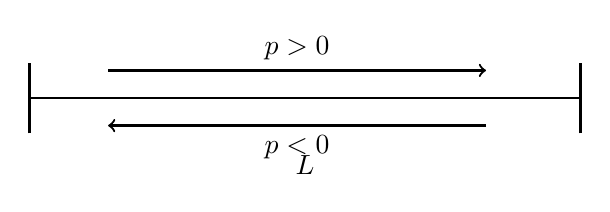
\begin{tikzpicture}[x=1cm,y=1cm]
\draw[thick] (0,0) -- (7,0);
\draw[very thick] (0,-0.45) -- (0,0.45);
\draw[very thick] (7,-0.45) -- (7,0.45);
\draw[->,thick] (1.0,0.35) -- (5.8,0.35) node[midway,above]{\(p>0\)};
\draw[->,thick] (5.8,-0.35) -- (1.0,-0.35) node[midway,below]{\(p<0\)};
\draw (3.5,-0.85) node{\(L\)};
\end{tikzpicture}
\caption{有限線段兩端的反射會使行波的動量反向。}
\end{figure}

還有另一種讓系統有限、同時保留動量守恆的方法：將線段的兩個端點視為同一點。可以把結果畫成一個圓，但不需要真的有一個嵌在二維空間中的圓。數學上的意思很簡單：座標具有週期性，走過總長度 \(L\) 後，就會回到同一點。

\begin{figure}[t]
\centering
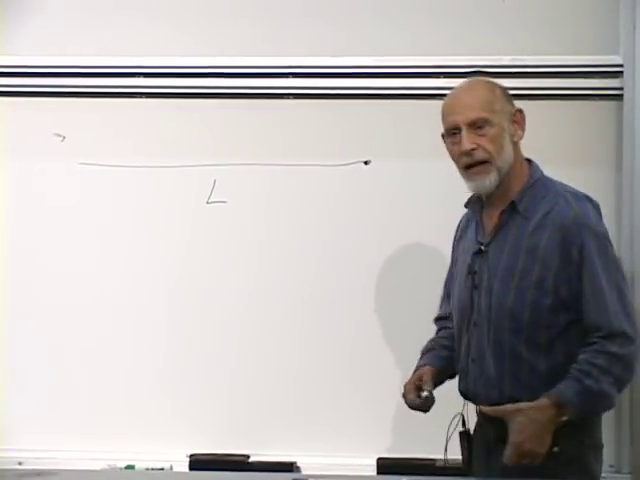
\includegraphics[width=0.72\textwidth]{lecture_02_figure_06.png}
\caption{總長度為 \(L\) 的一維路徑，用以介紹週期性識別。}
\lectureframe{00:51:21}
\end{figure}

下方示意圖明確呈現端點識別。\footnote{示意圖參照 00 至 51 的週期性識別論證：09--00至52：37。}

\begin{figure}[t]
\centering
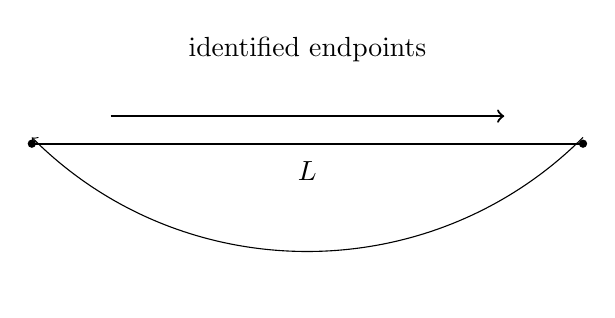
\begin{tikzpicture}[x=1cm,y=1cm]
\draw[thick] (0,0) -- (7,0);
\fill (0,0) circle (1.5pt);
\fill (7,0) circle (1.5pt);
\draw[->,thick] (1.0,0.35) -- (6.0,0.35);
\draw (3.5,-0.35) node{\(L\)};
\draw[->,bend left=45] (7,0.08) to (0,0.08);
\draw (3.5,1.2) node{identified endpoints};
\end{tikzpicture}
\caption{將長度為 \(L\) 的路徑兩端識別後形成的週期性一維空間。}
\end{figure}

向右移動的波接著抵達圖示端點，從起點重新出現，並繼續向右移動。向左移動的波也會繼續向左。由於沒有特定端點讓波反射，動量便不會反向。週期性空間使體積有限且保留動量，但也帶來一項重要結果：允許的動量是離散的。

總長度內必須容納整數個波長。對非定值模式而言，
\begin{equation}
\lambda_{|N|}=\frac{L}{|N|},
\qquad |N|=1,2,3,\ldots .
\end{equation}
因此波長的大小可以是 \(L\)、\(L/2\)、\(L/3\) 等。像 \(L/\sqrt{2}\) 這樣的選擇便不符合條件：波繞行一圈後會以錯誤的相位返回，無法與起始值相接。

利用 \(p=h/\lambda\)，第 \(|N|\) 個非定值模式的動量大小為
\begin{equation}
|p_N|=\frac{|N|h}{L}.
\end{equation}
若要毫無歧義地涵蓋兩個傳播方向和定值模式，將模式標記設為正負皆可會較方便：
\begin{equation}
p_N=\frac{Nh}{L},
\qquad N=0,\pm1,\pm2,\ldots .
\end{equation}
\(N\) 為正或負，代表相反的傳播方向。\(N=0\) 模式為定值模式，動量為零；它沒有有限波長可代入 \(h/\lambda\)。因此，基本動量間距為 \(h/L\)。

對宏觀的 \(L\) 而言，\(h\) 和 \(1/L\) 都使動量間距極小，因此允許值非常密集，看起來幾乎連續。然而，受限於圓形金屬線上運動的珠子，仍恰好具有這種離散譜。

\begin{classroomqa}
\lecturetimestamp{00:58:27}
\audiencequestion{量子化的是波的總動量，還是與單一週期相關的動量？}
\lecturerresponse{這項敘述適用於每個量子的動量。每個量子的動量都必須是允許的離散值之一。因此，任意一群量子的總動量也會是基本單位 \(h/L\) 的整數倍。}
\end{classroomqa}

\begin{classroomqa}
\lecturetimestamp{00:59:22}
\audiencequestion{為什麼波繞行一圈後必須回到相同的值？}
\lecturerresponse{識別後的兩個端點是同一個物理位置，因此可觀測的場在該處必須具有相同的值。若兩側不匹配，場在該處就會突然跳變。這種不連續性需要付出很大的能量與動量代價；可容許的場組態必須連續且具有週期性。}
\end{classroomqa}

\begin{classroomqa}
\lecturetimestamp{01:00:09}
\audiencequestion{如果波局域成一個波包，會怎麼樣？}
\lecturerresponse{波包是平面波的傅立葉和，也可以說是正弦波與餘弦波的傅立葉和。在週期性空間中，這個和只能包含允許的離散動量模式。因此，量子化的敘述適用於每個可容許波包的傅立葉分量。}
\end{classroomqa}

\begin{classroomqa}
\lecturetimestamp{01:01:01}
\audiencequestion{週期長度 \(L\) 極小時會出問題嗎？}
\lecturerresponse{隨著 \(L\) 減小，基本動量 \(h/L\) 會變得非常大。在一般微觀尺度下，這不會立即造成矛盾；但若試圖將這個建構推至普朗克長度尺度，預期就需要新的物理。}
\end{classroomqa}

現在將圓形圖像按字面理解：一顆珠子在半徑為 \(r\) 的圓形金屬線上運動，圓周長為 \(L=2\pi r\)。允許的切向動量為
\begin{equation}
p_N=\frac{Nh}{2\pi r}=\frac{N\hbar}{r}.
\end{equation}
對於沿圓形軌道運動的非相對論粒子，角動量為 \(mvr\)。由於在這種情況下 \(p=mv\)，所以角動量就是 \(rp\)。表示式 \(mvr\) 並非相對論情況下的通用形式，因為此時 \(p\) 不再只是 \(mv\)；但動量乘以垂直距離仍是正確的關係。以向量表示，\footnote{講課時先用 \(L\) 表示角動量，隨後發現它與週期長度的符號 \(L\) 相衝突，於是改用了其他符號。這裡一律使用 \(J\)；參見 01：03：40--01：05：21。}
\begin{equation}
\vec J=\vec r\times\vec p,
\end{equation}
切向圓周運動的角動量大小為 \(J=rp\)。因此
\begin{equation}
J_N=rp_N=N\hbar.
\end{equation}
線動量的間距取決於圓的大小，但角動量的單位永遠是 \(\hbar\)。涉及費米子時，整數規則會有例外；這些例外留待之後討論。

接下來要更精確地連結場、粒子和量子。這需要簡短回顧算符與簡諧振子的量子力學。

\section{波模式與量子算符}

接下來的量子力學內容必然較為抽象，目的在於複習。簡諧振子是核心系統，因為波就是一種振盪。在固定位置上，電場、磁場或任何其他波振幅都會隨時間週期性變化；說一個分量具有頻率，就等於說它正在振盪。

一般的波不一定只有一個波長。不同顏色的光可以混合在一起；反過來說，稜鏡也可以把混合光分解成各種組成色，牛頓分解白光就是一例。每個分量都有自己的波長、頻率、振幅、能量和動量。因此，混合波可以分解為具有不同能量和動量的量子。每個波長決定一個頻率，而每個定頻分量的行為都像一個振子。這就是為什麼場的自然基本單元是簡諧振子，而不是任意的量子系統。

量子可觀測量以算符表示。算符可以相加、相乘；但與普通數不同，算符乘積不一定與相乘順序無關。設\(A\)和\(B\)代表系統的兩種性質，各自都可能單獨測量。例如，\(A\)可能代表電場，\(B\)可能代表磁場。若測得的數值是普通數\(a\)和\(b\)，則
\begin{equation}
ab=ba.
\end{equation}
它們的數值乘積不可能因相乘順序而異。然而在量子力學中，相應的算符卻可能滿足\(AB-BA\neq0\)。

乍看之下，這似乎說不通。如果測量電場得到一個數，測量磁場得到另一個數，那麼這兩個數相乘，無論順序如何，結果都必須相同。解決之道在於：若算符乘積會因順序而異，這兩個量就不能同時測量。測量其中一個的實驗會干擾另一個量的測量。這並不矛盾，因為這兩個數值無法同時取得。

若兩個量可以同時測量，測得的數值就是普通數，而普通數彼此對易。因此，判斷能否同時測量的條件是對易子
\begin{equation}
[A,B]=AB-BA.
\end{equation}
對易子為零表示這些可觀測量彼此相容；對易子不為零則表示相應的測量會互相干擾。對調兩項的順序，符號便會反轉：
\begin{equation}
[B,A]=-[A,B].
\end{equation}

對非相對論粒子而言，三個位置分量彼此對易，三個動量分量也彼此對易：
\begin{align}
[x,y]&=[y,z]=[z,x]=0,\\
[p_x,p_y]&=[p_y,p_z]=[p_z,p_x]=0.
\end{align}
三個座標可以同時確定，三個動量分量也可以同時確定。相應的位置分量與動量分量則不對易：
\begin{equation}
[x,p_x]=[y,p_y]=[z,p_z]=i\hbar,
\end{equation}
而像\([x,p_y]\)這樣的混合分量則為零。測量位置座標會使粒子的共軛動量受到擾動。等價地說，相應的位置與動量不確定度之積受\(\hbar\)所限制。

\begin{classroomqa}
\lecturetimestamp{01:16:30}
\audiencequestion{從\(x\)變換到\(y\)時，對易子中的\(i\)是否也應該變成\(j\)？}
\lecturerresponse{不會。符號\(i\)始終表示虛數單位，也就是負一的平方根。它既不是笛卡兒單位向量的標記，也不是四元數符號\(i,j,k\)之一。}
\end{classroomqa}

\begin{classroomqa}
\lecturetimestamp{01:17:24}
\audiencequestion{\(AB-BA\)是否表示先測量\(A\)，再測量\(B\)，然後把測量順序反過來？}
\lecturerresponse{不是。這兩項是算符或矩陣依不同代數順序相乘的結果，並不表示實際的測量先後次序。它們與不相容測量之間的關聯，是算符代數的結果，而不是這種乘積的定義。}
\end{classroomqa}

\begin{classroomqa}
\lecturetimestamp{01:18:32}
\audiencequestion{這些位置--動量對易關係可以直接套用在光子上嗎？}
\lecturerresponse{不能直接套用。這些關係適用於非相對論粒子，而且形式簡潔。光子的位置較難定義，因此類似的敘述需要更謹慎處理；這裡也不需要用到。}
\end{classroomqa}

\section{量子簡諧振子}

彈簧上的重物、聲波和光波都是振盪運動的例子。每個理想簡諧振子都有一個頻率。對於彈簧而言，一個完整週期不只是重物回到同一位置所需的時間；它還必須朝同一方向運動。每秒完整週期的次數是\(f\)，而\(\omega=2\pi f\)。

在古典力學中，理想振子可以具有任意非負能量。輕推一下會有較小的能量，用力推則會有較大的能量。真實的彈簧終究會斷裂或熔化，但數學上的理想化模型具有連續的正能量範圍。量子振子則不同：它允許的能量形成離散且等間距的階梯。將能量原點選在最低能階，使其能量定為零，
\begin{equation}
E_n=n\hbar\omega,
\qquad n=0,1,2,\ldots .
\end{equation}
等間距的能階可以如下圖示。\footnote{能階示意圖依據01的板書討論：21：20--01：23：56。}

\begin{figure}[t]
\centering
\begin{tikzpicture}[x=1cm,y=0.9cm]
\draw[->] (0,0) -- (0,5.35);
\draw (0,5.5) node[above]{energy};
\foreach \y/\lab in {0.6/{0},1.6/{\hbar\omega},2.6/{2\hbar\omega},3.6/{3\hbar\omega},4.6/{n\hbar\omega}}
{
  \draw[thick] (0.2,\y) -- (2.2,\y);
  \draw (-0.25,\y) node[left]{\(\lab\)};
}
\draw[->,thick] (2.8,0.68) -- (2.8,1.52);
\draw (3.2,1.1) node[right]{\(a_+\)};
\draw[->,thick] (3.7,1.52) -- (3.7,0.68);
\draw (4.1,1.1) node[right]{\(a_-\)};
\end{tikzpicture}
\caption{採用約定\(E_n=n\hbar\omega\)時，等間距的振子能階。}
\end{figure}

能階間距\(\hbar\omega\)，正是先前賦予角頻率為\(\omega\)之單一光子的能量。數值\(2\hbar\omega\)可以是頻率為\(2\omega\)的振子中一個量子的能量，也可以是頻率為\(\omega\)的振子中兩個量子的能量。這裡需要的是第二種解讀。單一固定頻率的振子可以含有零個、一個、兩個、三個或更多量子，而相鄰能階之間沒有其他允許的能量。

整數\(n\)用來標記振子態，記作右矢\(|n\rangle\)。態\(|0\rangle\)是基態，態\(|1\rangle\)有一個激發量子，態\(|2\rangle\)有兩個，依此類推。右矢只是表示算符所作用之態的記號。

定義升算符\(a_+\)，使態上升一個能階；再定義降算符\(a_-\)，使態下降一個能階：
\begin{align}
a_+|n\rangle &= \sqrt{n+1}\,|n+1\rangle,\\
a_-|n\rangle &= \sqrt{n}\,|n-1\rangle.
\end{align}
數值平方根因子是定義的一部分。作用在最低能態時，
\begin{equation}
a_-|0\rangle=0,
\end{equation}
因為基態以下沒有其他態。

這裡必須區分普通數與算符。標記\(n\)和\(\sqrt n\)之類的係數都是普通數，與所有量都對易。符號\(a_+\)和\(a_-\)則是算符，必須保留其順序。

先讓\(|n\rangle\)降低，再將它升高。降低這一步得到
\begin{equation}
a_-|n\rangle=\sqrt n\,|n-1\rangle.
\end{equation}
接著以\(a_+\)作用於所得的態，會再帶來一個因子\(\sqrt n\)，因為將\(|n-1\rangle\)升高會回到\(|n\rangle\)：
\begin{align}
a_+a_-|n\rangle
&=a_+\bigl(\sqrt n\,|n-1\rangle\bigr)\\
&=\sqrt n\,\sqrt n\,|n\rangle\\
&=n|n\rangle.
\end{align}
因此，\(a_+a_-\)會讀出能階標記。例如，假設已知\(|\chi\rangle\)是數算符的本徵態，但不知道它的能階標記。若
\begin{equation}
a_+a_-|\chi\rangle=q|\chi\rangle,
\end{equation}
那麼普通數值係數\(q\)就是該態中的量子數。因此，這個乘積就是數算符：
\begin{equation}
\hat n=a_+a_-,
\end{equation}
在所選的能量約定下，哈密頓量為
\begin{equation}
H=\hbar\omega\,a_+a_-.
\end{equation}
事實上，對任一能階作用都會得到\(H|n\rangle=n\hbar\omega|n\rangle\)。

現在將順序反過來。先升高，得到\(\sqrt{n+1}|n+1\rangle\)。接著降低，便回到\(|n\rangle\)，並帶來第二個因子\(\sqrt{n+1}\)：
\begin{align}
a_-a_+|n\rangle
&=a_-\bigl(\sqrt{n+1}\,|n+1\rangle\bigr)\\
&=\sqrt{n+1}\,\sqrt{n+1}\,|n\rangle\\
&=(n+1)|n\rangle.
\end{align}
這兩種順序對每個態的作用相差一，因此
\begin{equation}
[a_-,a_+]=a_-a_+-a_+a_-=1.
\end{equation}

振子還有振幅和相位。相位指出振子在振盪週期中所處的位置；具體而言，可以用振子沿選定方向通過原點的時刻來確定相位。延後通過原點的時刻會改變相位，但不會改變頻率。階梯算符把與振幅和相位相關的量子變數組合起來。這套代數本質上是量子的，但算符的作用很簡單：\(a_+\)增加一個振子的能量量子，\(a_-\)則移除一個。對電磁模式而言，這些量子就是光子，因此這兩個算符稱為產生算符和湮滅算符。

\begin{classroomqa}
\lecturetimestamp{01:37:34}
\audiencequestion{升算符和降算符代表某種物理測量嗎？}
\lecturerresponse{光子數可以測量。由於其他技術上的原因，算符\(a_+\)和\(a_-\)本身並不是可測量的可觀測量。它們的對易子顯示兩者不對易，但單憑這一點，並不能論證其中任一算符本身不可觀測。}
\end{classroomqa}

具有不同固有頻率的一組彈簧，對應許多彼此獨立的振子。空腔中的電磁模式也是如此：可以激發某一波長的模式，而不必讓其他模式具有相同的激發。在量子力學中，每個獨立振子都有產生算符和湮滅算符，分別增加和移除其中固定頻率的量子。這套描述很重要，因為粒子將被辨認為正是這些量子。

\section{將場視為振子的集合}

回到總長度為\(L\)的週期性一維空間。其非常數模式的波長大小為
\begin{equation}
\lambda_N=\frac{L}{N},
\qquad N=1,2,3,\ldots ,
\end{equation}
相應的角頻率為非負值\(\omega_N\)。為了與先前的動量譜比較，可以將帶正負號的整數重新標記為\(M\)：
\begin{equation}
p_M=\frac{Mh}{L},
\qquad M=0,\pm1,\pm2,\ldots .
\end{equation}
\(M\)的正負號記錄傳播方向。
\editorialnote{在01：42：08--01：42：24處，頻率模式的索引已由帶正負號的範圍修正為從零起算的非負範圍。此處使用符號\(M\)，只是為了將帶正負號的動量記號與非負的頻率模式標記\(N\)區分開來；這並不表示\(+M\)和\(-M\)各自有獨立的佔據數。非常數振子列表從\(N=1\)開始。}

每個允許的頻率都會像一個簡諧振子。能量可以先獨立地加入某個頻率的模式，再加入另一個頻率的模式。量子場的第一個詳細例子留待下一講討論，但態的記號已經很清楚。將非常數模式由最長波長開始依序排列，寫成
\begin{equation}
|n_1,n_2,n_3,\ldots\rangle,
\end{equation}
其中\(n_N=0,1,2,\ldots\)表示頻率為\(\omega_N\)的振子所含的量子數。第一個分量表示最長波長模式中有多少個量子，第二個分量表示下一個模式中有多少個量子，依此類推，無窮延續。

弦的諧波可以讓這個建構更具體。從基頻到接下來兩個諧波的變化如下圖所示。\footnote{此示意圖依據01：45：20--01：47：46處關於弦諧波的討論。}

\begin{figure}[t]
\centering
\resizebox{\linewidth}{!}{%
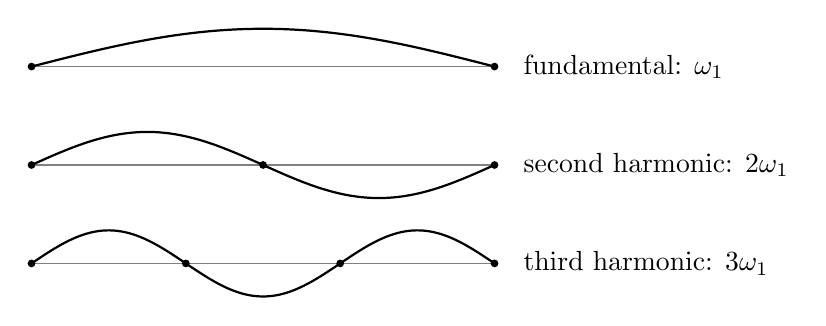
\begin{tikzpicture}[x=0.98cm,y=1cm]
\draw[gray] (0,2.5) -- (6,2.5);
\draw[thick] plot[domain=0:6,samples=120] (\x,{2.5+0.48*sin(30*\x)});
\fill (0,2.5) circle (1.4pt);
\fill (6,2.5) circle (1.4pt);
\node[right] at (6.25,2.5) {fundamental: \(\omega_1\)};

\draw[gray] (0,1.25) -- (6,1.25);
\draw[thick] plot[domain=0:6,samples=120] (\x,{1.25+0.42*sin(60*\x)});
\fill (0,1.25) circle (1.4pt);
\fill (3,1.25) circle (1.4pt);
\fill (6,1.25) circle (1.4pt);
\node[right] at (6.25,1.25) {second harmonic: \(2\omega_1\)};

\draw[gray] (0,0) -- (6,0);
\draw[thick] plot[domain=0:6,samples=120] (\x,{0.42*sin(90*\x)});
\fill (0,0) circle (1.4pt);
\fill (2,0) circle (1.4pt);
\fill (4,0) circle (1.4pt);
\fill (6,0) circle (1.4pt);
\node[right] at (6.25,0) {third harmonic: \(3\omega_1\)};
\end{tikzpicture}%
}
\caption{弦的基頻、第二諧波和第三諧波，分別具有零個、一個和兩個內部節點。}
\end{figure}

基頻振動時形成一個寬廣的弧形，沒有內部節點。它是一個振子，可以含有\(n_1=0,1,2,\ldots\)個量子；每個激發量子的能量為\(\hbar\omega_1\)。第二諧波有一個內部節點，頻率是基頻的兩倍。如果基頻發出中央C音，這個模式就會發出高一個八度的C音。它有獨立的佔據數\(n_2\)，其中每個量子的能量為\(\hbar\omega_2=2\hbar\omega_1\)。第三諧波有兩個內部節點，頻率是基頻的三倍。它也有自己的獨立佔據數\(n_3\)，同樣可以是任何非負整數。

逐一考慮各個模式，在上述能量約定下，每個模式的能量等於其佔據數乘以量子能量。將各模式的能量加總可得
\begin{equation}
E=\sum_{N=1}^{\infty} n_N\hbar\omega_N.
\end{equation}
\editorialnote{這個求和式是將01：44：02--01：47：46處分別列出的模式能量，以代數形式加總而成。}

每個場模式都必須重做同一套簡諧振子計算，每個獨立振子各有一個產生算符和一個湮滅算符。在這個初步的基本圖像中，量子場就是整組振子，以及它們的產生--湮滅代數。

這套描述適用於粒子散射。具有確定能量和動量的量子進入實驗，具有其他能量和動量的量子則離開實驗。湮滅算符會移除入射粒子；出射粒子則由相應模式的產生算符加入末態。

\begin{classroomqa}
\lecturetimestamp{01:49:38}
\audiencequestion{同一個整數同時用來標記振子模式和計算其中量子的數目嗎？}
\lecturerresponse{這裡有兩個不同的整數。模式標記\(N\)指出空間圖樣；在弦的例子中，節點數決定頻率\(\omega_N\)。佔據數\(n_N\)則表示具有該頻率的量子有多少個。}
\end{classroomqa}